\section{Discussion and Analysis}
\label{sec:discussion}
In this section we discuss the implementation and performance analysis of HBLast on the target FPGA platforms.

\subsection{Implementation}
HBLast is implemented using Verilog HDL language targeting Xilinx FPGAs.
The HBLast core implementation is FPGA agnostic and can be directly ported to other FPGA platforms including Intel and Lattice.
The design is thoroughly simulated for its functional and timing correctness using Xilinx Vivado simulator.
Xilinx Vivado 2018.2 design suite is used for implementing the platform on the VC709 evaluation platform.
The VC709 evaluation board supports Virtex-7 XC7VX690T-2FFG1761C FPGA. 
Along with Vivado, AWS-FPGA HDK tool flow is used for implementing the design on the cloud instances.
The cloud FPGA instance is the Xilinx Ultrascale+ VU9P device supporting -2 speed grade.
\subsection{Resource utilization}
The module-wise and total resource utilization of the platform is reported in Table~\ref{tab:util}. 
On the Virtex-7 FPGA the platform HBLast consumes about 4.7\% of LUTs, 2.4\% of flip flops and 3\% of BRAMs.
The HBLast core does not consume any FPGA-architecture dependent resource such as BRAMs or DSP slices, which make them highly portable.
The BRAMs are utilized by the PCIe and DRAM controllers, which are specific to Xilinx FPGAs.
The implementation is very lite-weight enabling it to run at high clock frequencies.
On the Amazon F1 instance, the utilization is much lower since the PCIe and DRAM controllers are absent and are managed by the \emph{shell} logic.
The resource requirement of the shell logic is not reported in the table. 

\begin{table}[!t]
\caption {Resource utilization of HBLast when targeting on-premises and EC2 implementations} \label{tab:util}
\begin{tabular}{l|l|l|l}
\toprule
Module Name        & Slice LUTs & Slice Regs & Block RAM Tile \\
\midrule
\multicolumn{4}{c}{\bf VC709 Implementation}\\
\midrule
Hit                & 2958       & 808        & 0              \\
Expand             & 2342       & 2410       & 0              \\
bridge             & 107        & 1253       & 0              \\
memoryInt          & 5321       & 4809       & 0              \\
\midrule
{\bf HBLast}       & 5428      & 6062        & 0              \\
u\_mig\_7series\_0 & 6002      & 4676        & 1              \\ 
Dyract             & 9065      & 10812       & 42             \\
\midrule
{\bf Total}        & 20495     & 21520       & 43             \\
\midrule
\multicolumn{4}{c}{\bf AWS EC2 F1 implementation}\\
\midrule
Hit                & 3134      & 1320       & 0               \\
Expand             & 2980      & 2451       & 0               \\
bridge             & 262       & 1254       & 0               \\
memoryInt          & 3165      & 4821       & 0               \\
\midrule
{\bf Total}        & 9541      & 9846       & 0               \\
\bottomrule
\end{tabular}
\label{tab:util}
\end{table}


\subsection{Performance analysis}

On both VC709 and F1 platforms, the HBLast core operates at 200MHz clock frequency provided by the DRAM memory controller.
The maximum performance of the implementation is limited by the performance of the memory sub-system. 
Since the implementation uses a 512-bit wide interface to the DRAM controller, running at 200MHz saturates the maximum supported DRAM bandwidth.
The PCIe interface runs at 250MHz, 256-bit wide interface supporting a maximum bandwidth of 8GB/s.
Since the database is stored only once the external DRAM during the system initialization, the bandwidth has little impact on overall system performance.
But scenarios where different databases are used in a time-multiplexed manner, this will be the bottleneck on the overall system performance.

The latency of the platform is measured as the duration between first read operation of the query and the completion of the search operation. 
When the device starts reading the register, where query is stored, it waits until the signal that indicates the validity of query comes. 
Once the \textit{queryValid} flag is high, the process of searching for the hits/matches is initiated, and it lasts until the end of the algorithm.  
In expansion process, if the exact match is found in the middle of the of 512-bits, that is there are at least 200 bits before or after the location of the match, the former or latter 512-bits of the database in DRAM are not retrieved. 
Otherwise, DRAM will be accessed one more time to retrieve the additional 512-bits to allow the range of expansion be sufficient for search operation. 

HBLast was examined under two scenarios to identify the dependence of latency on the characteristics of the search in database. 
The first scenario was to determine the relationship between the latency and the location of the exact match in the database.
In all the cases, the size of the HSP is 90-Wmers. 
As it is depicted in Fig.~\ref{fig:plot1}, X-axis represents the location of exact match in database, and Y-axis shows the corresponding time to complete the search. 
The matches are located in different 512-bits in database, thus the matches are found in only a certain read operation from the database. 
The first point in the plot in Fig.\ref{fig:plot1}, indicates the latency when the match is located in the first 512-bits of the database. 
The rest of the points represent that the matches are located in second, third, forth, fifth and sixth 512-bits of the database respectively. 
It could be seen that the latency for the first case (match in first 512-bits of database) differs from others. 
The latency in the first case is approximately 6.5 msec, and in the rest of cases it is roughly 8.6 msec. 
The difference in latency can be explained by the fact that, the first read operation from DRAM requires longer time due to precharging the particular row.
Subsequent read operations happen from the same row, thus causing lesser latency.
Data shows that there is a linear relation between the location of the first match and the total latency of operation.\\
\begin{equation}
\label{eq2}
Latency = 6.5 + 0.008*n~~milliSeconds
\end{equation}
Where n is the exact match position for 512-bit DRAM data.
This also shows that the implementation takes only about 8us for processing a 512-bit (256 letter) sequence.
This performance is far superior than existing software implementations.

\begin{figure}
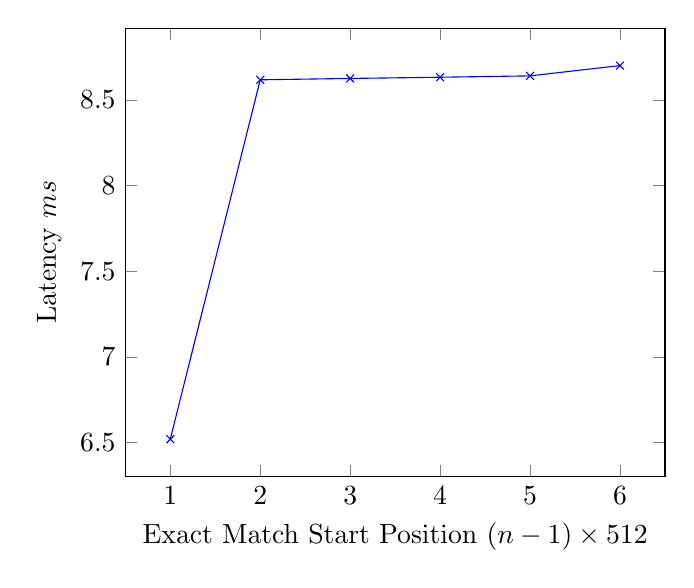
\begin{tikzpicture}
	\begin{axis}[
		xlabel=Exact Match Start Position $(n-1)\times 512$,
		ylabel=Latency $ms$]
	\addplot[color=blue,mark=x] coordinates {
		(1,6.52)
		(2,8.617)
		(3,8.625)
		(4,8.632)
		(5,8.64)
		(6,8.70)
	};
	\end{axis}
\end{tikzpicture}
\caption{Relationship between latency and position of exact match of sequence in database} \label{fig:plot1}
\end{figure}

The second scenario tests the relation between the latency and number of matches between the query and database. 
It could be seen from Fig.\ref{fig:plot2} that the latency linearly increases with the number of matches.
The steep increase between the first two data points is due to same DRAM access latency described in the previous section.

\begin{figure}
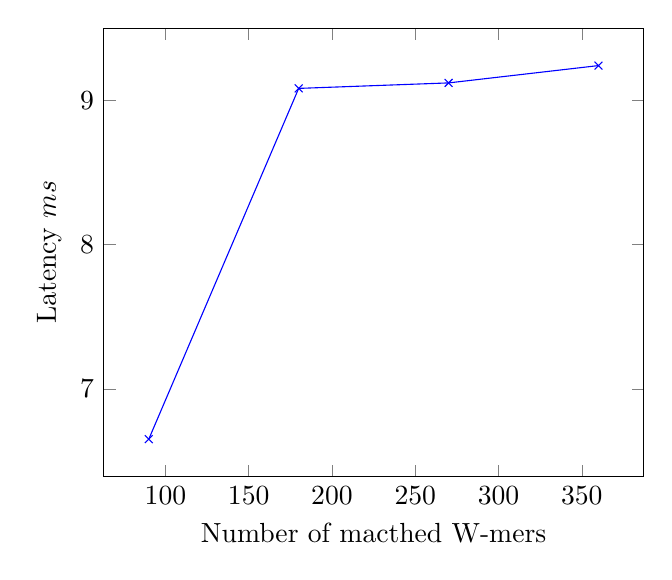
\begin{tikzpicture}
	\begin{axis}[
		xlabel=Number of macthed W-mers,
		ylabel=Latency $ms$]
	\addplot[color=blue,mark=x] coordinates {
		(90,6.652)
		(180,9.082)
		(270,9.12)
		(360,9.24)
	};
	\end{axis}
\end{tikzpicture}
\caption{Relationship between latency and number of exact match of sequence in database} \label{fig:plot2}
\end{figure}

\subsection{Comparison with the state of the art}
The word scanning speed in Mercury BLASTn is 96 M matches/s and that of Multiengine BLASTn Accelerator is 6400 M matches/s. 
The latest systolic array-based implementation achieves 14450 M matches/s through a multiple hit detection unit~\cite{guo2012systolic}.
HBLast is capable to achieving 49200 M matches/s due to its 240 parallel comparators running at 200MHz clock frequency.

The latest reported average latency for software and hardware implementation of BLASTp algorithm for random 256-character long query searching in a 188719038-character long database is 3087ms and 1058ms respectively~\cite{guo2012systolic}.
This work does not report best- and worst-case latencies and the average case is found only by running 15 random query sequences.
HBLast requires only 360MB DRAM space for storing this database since each character is represented only using 2 bits.
The best and worst-case latencies for HBLast in this case are 6.5ms and 5900ms respectively.
The average values could not be directly compared in this case, since the exact queries used for testing is not reported in the literature.